\chapter{Semantičko poređenje opštih AST}
\label{chp:ASTComparing}

Jedna od motivacija svođenja imperativnih jezika na isti nivo apstrakcije (opisane u poglavlju \ref{sec:MyAST}) može biti poređenje kodova pisanih u različitim programskim jezicima. Pritom, s obzirom da su u pitanju stabla, moguće je koristiti razne algoritme za poređenje stabala (ali i grafova uopšte) nad ovakvim apstrakcijama. Pritom, potrebno je i definisati kriterijum poređenja --- moguće je porediti kodove \emph{strukturno}, \emph{semantički} itd. U ovom radu je od značaja semantička ekvivalentnost, koja je u opštem slučaju neodlučiv problem. Međutim, ukoliko se ograničimo samo na strukturno slične kodove, moguće je dobiti smislene rezultate u praksi, nalik na one dobijene u ovom radu. Precizna definicija strukturne sličnosti se obično iskazuje u terminima sličnosti strukture njihovih apstrakcija. Naravno, postoje kodovi koji nisu strukturno ekvivalentni ali su semantički ekvivalentni --- takvi slučajevi se onda neće razmatrati zbog neispunjenosti pretpostavke o strukturnoj sličnosti. 

Pretpostavka strukturne sličnosti je velika i znatno smanjuje broj slučajeva upotrebe takvog upoređivača. Međutim, danas je od velikog značaja verifikacija programa dobijenih sitnim refaktorisanjem već postojećh i verifikovanih programa, često ne menjajući strukturu uopšte (a ako se struktura koda menja onda se to obično radi u mmanjim koracima između kojih i dalje važi pretpostavka strukturne sličnosti kodova u susednim koracima). Slično, prepisivanja programa sa jednog programskog jezika na drugi su jako uobičajena, pa je i u takvim situacijama implicitno prisutna strukturna slučnost, što zavisi od konkretnih programskih jezika ali se u praksi često smanjuje napor tako što se održava struktura koda, barem u inicijalnim verzijama. 

Definicija strukturne sličnosti za potrebe ovog rada će se odnositi na sličnosti u rasporedu blokova naredbi dok će raspored naredbi u blokovima biti nebitan. Na primer, ukoliko se prvi program sastoji od bloka naredbi u kome se nalaze dva druga bloka, očekuje se da i drugi program ima istu organizaciju blokova, pri čemu se pod terminom blok podrazumevaju i složene naredbe koje se sastoje od bloka naredbi u sebi, kao što su definicije funkcija, uslovna grananja, petlje i ostali tipovi složenih naredbi opisanih u \ref{subsec:MyASTStatementNodes}. Pod ovim uslovima, moguće je porediti blokove prvog programa sa odgovarajućim blokovima drugog programa.


\section{Simboličko izračunavanje}
\label{sec:Symbolics}

Današnji softver je veoma kompleksan i često funkcioniše na različitim nivoima arhitekture velikih projekata. Stoga je proces verifikacije softvera veoma značajan i delikatan. U procesu verifikacije se najčešće koriste ručno pisani testovi i pregledi koda od strane drugih programera. Uprkos svim ovim merama, greške su i dalje nezaobilazne --- jedan test može proveriti ponašanje koda za samo jedan ulaz. S obzirom da je nemoguće testirati sve ulaze zbog njihovog ogromnog broja (ukoliko posmatramo samo funkciju jedne promenljive koja prima 32-bitni ceo broj, broj mogućih ulaza je $2^{32}$) potrebno je da testovi dobro \emph{generalizuju} --- da pokrivaju opšte ali i neke specijalne ulaze. To se postiže uočavanjem da se vrednosti ulaza mogu razvrstati u klase po tome kakav izlaz uzrokuju. Ukoliko imamo funkciju koja deli dva broja, te klase mogu biti celi brojevi, realni brojevi, neke specijalne vrednosti specifične za operaciju deljenja (recimo $0$), kao i granice za tip podataka iz čijeg domena argumenti funkcije mogu uzeti vrednost. Čak i ovakav pristup, iako drastično smanjuje broj testova i eliminiše redundantne testove, i dalje zahteva relativno veliki broj testova u slučaju većih projekata i stoga je teško pronaći sve greške, pogotovo u slučajevima koji se retko dešavaju i ako ispoljavanje istih zavisi od stanja drugih komponenti ili pak nekih nedeterminističkih ponašanja samog sistema. Poželjno je čitav izvorni k\^od pokriti  testovima (engl. \emph{code coverage}) --- iako dostignuta pokrivenost koda od 100\% i dalje ne znači da taj k\^od ispravno radi.

\emph{Statička analiza koda} predstavlja analizu izvornog koda bez pokretanja istog sa ciljem ispitivanja stanja u kojima se može naći program i proveru rada jedinice koja se testira za mnogobrojne ulaze. Iako ispravna u teoriji, u praksi nailazi na puno problema --- osnovni je razlika u apstrakcijama koju prave statički analizator i programer.

\emph{Simboličko izvršavanje} \cite{SymbolicExecution} predstavlja sredinu između klasične verifikacije putem pisanja testova i statičke analize koda. Prilikom simboličkog izvršavanja, umesto stvarnih vrednosti ulaza koriste se \emph{simboličke promenljive}. Simbolička promenljiva nije vezana za specifičnu vrednost i analiza se dalje vrši samo nad njom --- samim tim se istovremeno mogu testirati višestruke klase sličnih ulaza. 

Primer simboličkog izvršavanja će biti opisan na isečku C koda sa slike \ref{fig:SymbolicExecCode}. Pretpostavimo da imamo deklarisanje promenljive \texttt{a}, \texttt{b} i \texttt{c} i da se neke operacije izvršavaju nad njima, reprezentovano komentarom u liniji $3$. U nekom trenutku se vrednosti tih promenljivih koriste kao uslovi od kojih zavisi prolaznost testa u poslednjoj liniji. Dodelimo svakoj promenljivoj simboličku vrednost --- \texttt{a = }$\alpha$, \texttt{b = }$\beta$, \texttt{c = }$\gamma$. Možemo izgraditi stablo izvršavanja i uslove koji moraju da važe nad simboličkim vrednostima $\alpha$, $\beta$ i $\gamma$ kako bi test u poslednjoj liniji prošao.

\begin{figure}[h!]
\begin{lstlisting}[language={}]
int a, b, c;

// ...

int x = 0, y = 0, z = 0;
if (a)      
    x = -2;
if (b < 5)  {
    if (!a && c)    
        y = 1;
    z = 2;
}

assert(x + y + z != 3);
\end{lstlisting}
\caption{Isečak C koda dat kao primer nad kojim će se prikazati simboličko izvršavanje.}
\label{fig:SymbolicExecCode}
\end{figure}

Ukoliko put izvršavanja programa zavisi od simboličke promenljive, kao što je to slučaj za izvorni k\^od sa slike \ref{fig:SymbolicExecCode}, simbolička promenljiva se konceptualno "grana" i analiza se nastavlja za oba slučaja posebno. Tako se dobija drvo izvršavanja, gde svaka putanja odgovara mnogim individualnim testovima koji bi uzrokovali prolazak izvršavanja tom putanjom. Vrednosti promenljivih u tim testovima moraju zadovoljiti uslove na kraju svake putanje --- tzv. \emph{uslove putanje} (engl. \emph{path conditions}). Odgovarajuće stablo izvršavanja za izvorni k\^od sa slike \ref{fig:SymbolicExecCode} sa definisanim simboličkim vrednostima $\alpha$, $\beta$ i $\gamma$ se može videti na slici \ref{fig:SymbolicExecTree}. Svaka naredba dodele je uokvirena pravougaonikom dok je uslov uokviren elipsom. Boje grana odgovaraju istinitosnoj vrednosti uslova iz poslednje linije u tom trenutku. Na kraju svake grane se nalazi uslov putanje za tu granu koje u nekim slučajevima može jedinstveno odrediti vrednost simboličke promenljive koja dovodi do prolaska tom putanjom ili u opštem slučaju generisati test primer koji dovodi do prolaska tom putanjom. Dakle, ukoliko je stablo simboličkog izvršavanja poznato, moguće je generisati kontra-primere koji pokazuju da program ne radi kao što je očekivano.

\begin{figure}[h!]
\centering
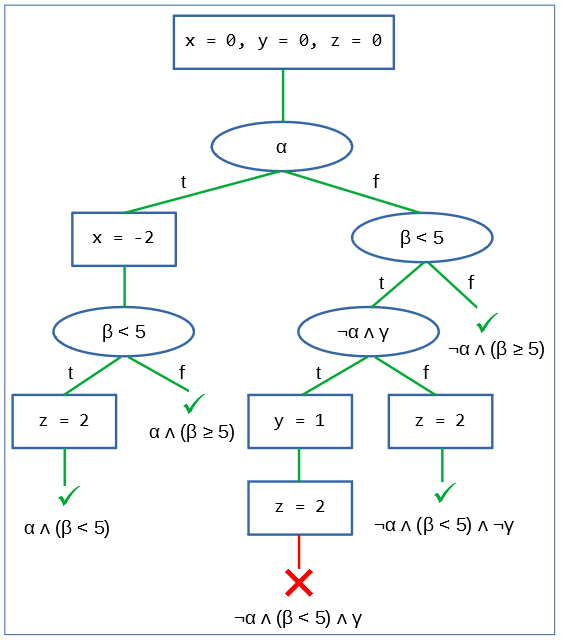
\includegraphics[scale=0.7]{images/sym_tree.png}
\caption{Drvo simboličkog izvršavanja na kom su prikazane sve putanje koje se razmatraju. Na kraju svake grane je napisan uslov koji mora da važi da bi se došlo do lista te grane.}
\label{fig:SymbolicExecTree}
\end{figure}

Simboličko izvršavanje, iako konceptualno moćno, ima par problema koji su uzrokovani pre svega kompleksnošću problema koji se rešava:
\begin{itemize}
    \item \emph{Eksplozija putanja} --- Broj putanja izvršavanja eksponencijalno zavisi od broja uslovnih grananja u kodu. Ukoliko imamo tri naredbe grananja, broj putanja izvršavanja je $2^3=8$. Štaviše, dovode do značajnog uvećanja broja stanja, jer ukoliko u petlji postoji uslov koji zavisi od simboličke vrednosti koja uzima vrednosti iz opsega 32-bitnog celog broja, broj putanja kroz petlju je u tom slučaju $2^{31}$, a u nekim slučajevima i beskonačan. Slično važi i za rekurziju.
    \item \emph{Ograničenja rešavača} --- Kako broj putanja raste, povećava se i broj uslova koji se moraju zadovoljiti prilikom nalaženja kontraprimera. U nekim slučajevima je moguće osloniti se na \emph{SMT rešavače} \cite{SMT} za nalaženje kontra-primera kako bi se ublažio ovaj problem.
    \item \emph{Modelovanje podataka} (engl. \emph{heap modelling}) --- Kreiranje simboličkih struktura podataka i pokazivača nije jednostavan proces.
    \item \emph{Modelovanje okruženja} (engl. \emph{environment modelling}) --- Nije uvek jednostavno adaptirati mehanizam za česte potrebe prilikom dizajna softvera kao što je korišćenje eksternih biblioteka i sistemskih poziva ali i specifičnosti sistema.
\end{itemize}

Postoji dosta alata i biblioteka koje pružaju interfejs za simboličko izračunavanje u raznim programskim jezicima --- jedan od najpoznatijih alata za simboličko izračunavanje je \emph{KLEE} \cite{KLEE}, izgrađen nad \emph{LLVM} infrastruktorom \cite{LLVM} \cite{LLVM04} i dizajniran za analizu koda pisanog u programskom jeziku C. U ovom radu je simboličko izvršavanje korišćeno za detekciju razlika u vrednostima promenljivih uz pomoć biblioteka za programski jezik C\#.

\section{Algoritam za semantičko poređenje}
\label{sec:ASTComparingAlgorithm}

U ovom radu je poređenje vršeno pomoću algoritma pisanog specifično za rad sa opštim apstrakcijama opisanim u \ref{sec:MyAST}. Grubi opis algoritma za poređenje, u daljem tekstu \emph{upoređivač}, je prikazan na slici \ref{fig:ComparisonAlgorithmPseudo}. Upoređivač se sastoji od više upoređivača koje porede specifične tipove čvorova. Za početak, potreban je jedan adapter koji će dobiti pokazivače na korene stabala koje je potrebno uporediti. S obzirom da tipovi čvorova mogu biti različiti, potrebno je proveriti da li su tipovi isti. Ukoliko to nije slučaj, prijavljuje se greška i rad se prekida. U protivnom, potrebno je odrediti tip čvorova i pozvati konkretni algoritam za poređenje. 

\begin{figure}[!h]
\begin{algorithmic}[1]
\Procedure{Uporedi}{$n_1$, $n_2$}
\If{\emph{$n_1$ i $n_2$ su istog tipa}}
    \State $t \gets$ \emph{tip čvora $n_1$}
    \If{\emph{postoji definisan upoređivač za čvorove tipa} $t$}
        \State $U \gets$ \emph{upoređivač čvorova tipa $t$}
        \State \textbf{return} U$(n_1, n_2)$
    \Else
        \If{$\text{BrojDece}(n_1) \neq \text{BrojDece}(n_2)$}d
            \State \textbf{return} \texttt{False}
        \Else        
            \If{$\text{Atributi}(n_1) \neq \text{Atributi}(n_2)$}
                \State \textbf{return} \texttt{False}
            \EndIf
            \For{$i \gets 0$ \textbf{to} $\text{BrojDece}(n_1)$}
                \State $d_1 \gets $ \emph{dete $i$ čvora $n_1$}
                \State $d_2 \gets $ \emph{dete $i$ čvora $n_2$}
                \If{\textbf{not} $\text{Uporedi}(d_1, d_2)$}
                    \State \textbf{return} \texttt{False}
                \EndIf
            \EndFor
            \State \textbf{return} \texttt{True}
        \EndIf
    \EndIf
\Else
    \State \textbf{return} \texttt{False}
\EndIf
\EndProcedure
\end{algorithmic}
\caption{Osnovni AST upoređivač.}
\label{fig:ComparisonAlgorithmPseudo}
\end{figure}

Podrazumevana implementacija poređenja može biti takva da se uporede atributi svih čvorova a zatim se svako dete prvog čvora rekurzivno uporedi sa odgovarajućim detetom drugog čvora (ukoliko imaju isti broj dece). Ako neki par dece nije ekvivalentan, onda to ne važi ni za njihove roditelje. Za većinu tipova čvorova ovakvo poređenje je dovoljno. 

Naredbe koje se sastoje od više drugih naredbi, kao što su npr.~definicije funkcija ili petlje, se moraju porediti drugačije jer složena naredba može sadržati lokalne promenljive. Niz naredbi koji predstavlja jednu složenu naredbu će u nastavku biti referisan pod terminom \emph{blok} ili \emph{blok naredbi}. Za poređenje blokova naredbi je stoga definisana posebna procedura poređenja opisana u nastavku.


\section{Upoređivač blokova naredbi}
\label{sec:ASTComparingBlocks}

Podrazumevani način poređenja dece svakog čvora nije dobar u opštem slučaju za blokove naredbi jer je osetljiv na izmene redosleda naredbi --- na primer promena redosleda deklaracija. Stoga je upoređivač blokova potrebno napisati tako da može da uoči semantičku ekvivalentnost iako naredbe nisu nužno jednake, a možda ih čak ima i različit broj.

Upoređivač se zasniva na poređenju vrednosti promenljivih na kraju svakog bloka naredbi. Apstrakcije dva programa se porede paralelno --- \emph{blok-po-blok}. Naredbe svakog bloka se izvršavaju i prate se izmene vrednosti promenljivih deklarisanih do tog trenutka (bilo u bloku koji se trenutno razmatra, ili u roditeljskim blokovima). Na kraju svakog bloka se vrši provera jednakosti simboličkih vrednosti promenljivih iz oba programa deklarisanih do tog trenutka i svaka razlika se prijavljuje kao potencijalna greška. Pošto broj promenljivih u programima ne mora biti isti iako su oni semantički ekvivalentni, za one promenljive koje nemaju parnjaka prilikom poređenja se prijavljuju upozorenja ali ne i greške ukoliko nije bilo konflikata prilikom poređenja vrednosti ostalih promenljivih. Upoređivač blokova naredbi je prikazan na slici \ref{fig:ComparisonAlgorithmBlocksPseudo}.

\begin{figure}[!h]
\begin{algorithmic}[1]
\Procedure{UporediBlokove}{$b_1$, $b_2$}
\State $gds_1 \gets $ \emph{simboli iz svih predaka bloka $b_1$}
\State $gds_2 \gets $ \emph{simboli iz svih predaka bloka $b_2$}
\State $lds_1 \gets $ \emph{lokalni simboli za blok $b_1$}
\State $lds_2 \gets $ \emph{lokalni simboli za blok $b_2$}
\State $\text{UporediSimbole}(lds_1, lds_2)$
\State $\text{IzvrsiNaredbe}(b_1, b_2, lds_1, lds_2, gds_1, gds_2)$
\State \textbf{return} $\text{UporediSimbole}(lds_1, lds_2) \wedge \text{UporediSimbole}(gds_1, gds_2)$
\EndProcedure
\end{algorithmic}
\caption{Upoređivač blokova naredbi.}
\label{fig:ComparisonAlgorithmBlocksPseudo}
\end{figure}

U opisu algoritma se koristi termin \emph{simbol} koji se sastoji od identifikatora i simboličke vrednosti promenljive. Lokalni simboli su deklarisani unutar bloka dok su globalni simboli deklarisani van trenutnog bloka a mogu se referisati iz njega. Pronalaženje deklarisanih simbola u bloku podrazumeva prolaz kroz naredbe bloka i registrovanje svih naredbi deklaracije, izvlačenje deklaratora iz njih i, uzimajući u obzir opcione inicijalizatore, kreiranje simboličke vrednosti za upravo deklarisani identifikator. Identifikator i opcioni simbolički inicijalizator čine \emph{simbol}. Isto se ponavlja za sve naredbe deklaracije u bloku i rezultat je skup deklarisanih simbola.

Nakon registrovanja svih lokalnih simbola proverava se njihova ekvivalentnost u funkciji \texttt{UporediSimbole}. Ova funkcija proverava da li se svi simboli iz prvog bloka nalaze u drugom i prijavljuje ukoliko neki simboli fale ili ukoliko postoje simboli koji su višak. Zatim, za simbole koji se nalaze u oba skupa, proverava njihove simboličke vrednosti. Ukoliko su te vrednosti različite, prijavljuje se potencijalna greška i na osnovu toga da li je bilo konflikata vraća se istinitosna vrednost. Razlog zašto se ta vrednost ne koristi dalje nakon prvog poziva ove funkcije je ta što različiti inicijalizatori ne znače nužno da postoji problem. Problem postoji ukoliko se nakon izvršavanja svih naredbi i dalje dešavaju konflikti u simboličkim vrednostima za neke promenljive. 

Procedura \texttt{IzvrsiNaredbe} izvršava paralelno naredbe iz oba bloka i na osnovu toga koje su naredbe u pitanju može i da ažurira simboličke vrednosti unutar skupova deklarisanih simbola. Pseudokod ove procedure je dat na slici \ref{fig:ComparisonAlgorithmBlocksPseudo1}. Naredbe se za svaki blok izvršavaju dok se ne naiđe do naredbe iz koje se može izvući novi blok --- to mogu biti naredbe grananja, iteracije, definicije funkcija i slično. Sve naredbe do pronađene naredbe se izvršavaju. Procedura \texttt{IzvrsiNaredbu} će proveriti tip naredbe i, u zavisnosti od toga da li je to naredba dodele, eventualno promeniti vrednosti u skupovima prosleđenih simbola. Nakon izvršavanja svih naredbi do pronađene naredbe koja sadrži blok, izvlači se blok iz nje (to isto se radi i za drugi program). Kad se blokovi izvuku, rekurzivno se poziva upoređivač blokova za pronađene parnjake. Po povratku iz rekurzivnog poziva nastavlja se isti postupak sve dok se ne izvrše sve naredbe. Pritom, algoritam se oslanja na strukturnu sličnost --- ukoliko jedan AST ima više blokova na istoj dubini u odnosu na drugi, poređenje možda neće uočiti neke razlike jer neki blokovi neće imati svog parnjaka ili njihovo uparivanje nije jednoznačno. 

Takođe je važno napomenuti da procedura \texttt{IzvrsiNaredbe} vraća povratnu vrednost koja se u algoritmu sa slike \ref{fig:ComparisonAlgorithmBlocksPseudo} ignoriše. Razlog za to je što, u nekim slučajevima, iako su unutrašnji blokovi naredbi različiti, želimo ipak da proverimo vrednosti promenljivih pre nego što zaključimo da postoji problem. Ukoliko, doduše, samo poredimo par čvorova složenih naredbi koje se sastoje od više jednostavnijih naredbi, u tom slučaju ćemo iskoristiti povratnu vrednost ove procedure jer ne postoji širi kontekst iz kojeg pozivamo ovu proceduru.

\begin{figure}[!h]
\begin{algorithmic}[1]
\Procedure{IzvrsiNaredbe}{$b_1$, $b_2, lds_1, lds_2, gds_1, gds_2$}
\State $n_1 \gets $ \emph{niz naredbi bloka $b_1$} 
\State $n_2 \gets $ \emph{niz naredbi bloka $b_2$}
\State $i \gets j \gets 0$
\State $ni \gets nj \gets 0$
\State $eq \gets $ \texttt{True}
\While{\texttt{True}}
    \State $ni \gets $ \emph{indeks prve naredbe koja sadrži blok u $n_1$ počev od indeksa $ni$}
    \State $nj \gets $ \emph{indeks prve naredbe koja sadrži blok u $n_2$ počev od indeksa $nj$}
    \For{$naredba \in \{n_1[x] \mid x \in [i..ni]\}$}
        \State $\text{IzvrsiNaredbu}(naredba, lds_1, gds_1)$
    \EndFor
    \State $i \gets i + ni$
    \For{$naredba \in \{n_2[x] \mid x \in [j..nj]\}$}
        \State $\text{IzvrsiNaredbu}(naredba, lds_2, gds_2)$
    \EndFor
    \State $j \gets j + nj$
    \If{$i > \text{Duzina}(n_1) \vee j > \text{Duzina}(n_2)$}
        \State \textbf{prekini petlju}
    \EndIf
    \State $nb_1 \gets $ \emph{izvuci blok iz naredbe $n_1[i]$}
    \State $nb_2 \gets $ \emph{izvuci blok iz naredbe $n_2[j]$}
    \State $eq \gets eq \wedge \text{UporediBlokove}(nb_1, nb_2)$
    \State $i \gets i + 1$
    \State $j \gets j + 1$
\EndWhile
\State \textbf{return} $eq$
\EndProcedure
\end{algorithmic}
\caption{Upoređivač blokova naredbi.}
\label{fig:ComparisonAlgorithmBlocksPseudo1}
\end{figure}

